\chapter{Neutron Diffusion Results}
\label{ch:diffusionResults}

\section{Introduction}
  The implementation of the \gls{fem} in this work has been compared
  against standard benchmark problems as well as analytic solutions to the
  multigroup neutron diffusion equation. Comparison against benchmark problems
  demonstrates an ability to solve problems for which this work was intended.
  Comparison against analytic solutions allows for more detailed error and
  convergence analysis as not only the system $\keff$ but also the flux solution
  is known exactly. 

  These comparisons serve as a verification of this implementation of the
  \gls{fem}. The verification strategy employed in this work is developed by
  \textcite{oberkampf}. The first step is ``code verification.'' Code
  verification compares computational results to exact analytic or manufactured
  results. Code verification serves to demonstrate that the code itself is
  solving the equations correctly as designed and with quantified numerical
  errors. This will be demonstrated with convergence to the analytic answer at
  the expected rate. The second step is ``solution verification.'' Solution
  verification compares computational results to benchmark results for the
  intended application of the solver. These benchmarks may have been been
  calculated computationally via another method or may come from experimental
  data. Whereas analytic solutions are known exactly, the data of benchmarks is 
  not exact. Typically, the benchmark solution has been verified by others 
  previously.

\section{Error Analysis}
  For all benchmark and analytic problems solved, a convergence study is 
  presented. An error vector is defined as $\ve = \phi(\vr) - \phi_{FEM}$ where
  $\phi_{FEM}$ is the solution to the \gls{fem} system of equations. 
  The error is then considered in terms of both \gls{rms} error calculated as 
  \begin{equation} 
    \label{eq:rms}
    \text{\gls{rms}}(\ve) = \sqrt{\frac{1}{N} \sum_{i=1}^{N} e_i^2},
  \end{equation}
  and error is considered in the maximal norm calculated as
  \begin{equation} 
    \label{eq:infnorm}
    \|\ve\|_{\infty} = \max_{i=1,2,\ldots,N} \lvert e_i \rvert.
  \end{equation}

  It has been shown that for a bounded second spatial derivative 
  within the problem domain, the \gls{fem} with linear elements as derived in 
  \chref{ch:neutronDiffusion} is second-order convergent in space 
  \cite{textbookli}. This implies the error in the maximal norm defined in 
  \eref{eq:infnorm} is bounded as
  \begin{equation} 
    \label{eq:error_bound}
    \|\ve\|_{\infty} \le c h^2 \| \grad^2 \phi(\vr) \|_{\infty}
  \end{equation}
  where $\ve$ is the error vector, $h$ is the characteristic mesh size, and $c$
  is a constant. \eref{eq:error_bound} implies that if the characteristic mesh 
  size is halved, the error is quartered. This relationship is useful as a 
  proper implementation of the \gls{fem} must converge to the correct answer and 
  do so at the correct rate.
  
  Mesh refinement studies are presented herein. For each refinement, $h$ is 
  halved by introducing new elements and placing new nodes at the midway point
  between existing nodes. Let $i$ be the refinement index and the refinement 
  ratio for a second-order convergent method is 
  \begin{equation}
    4 = \frac{e^{(i-1)}}{e^{(i)}}
  \end{equation}
  such that for some error quantity $e$, the error should theoretically decrease 
  by a factor of four for each refinement. As these are numerical solutions, the
  ratio rarely equals exactly four. It is observed that a few refinements are
  often necessary before the convergence reaches the asymptotic regime and the
  ratio approaches the expected value. This is especially the case when the
  second derivative is not bounded in problems with heterogeneous materials.
  
  For analytic solutions, the error of the function $\phi(\vr)$ itself can be 
  analyzed because the solution is known exactly. The derivations of the exact 
  solutions are presented in \apref{ap:analyticSolutions}. Both RMS errors and
  maximal norm errors are presented. It is observed that the RMS error
  refinement ratio approaches the expected value of four before the maximal
  error refinement ratio because the RMS error is an integral quantity over the
  problem domain whereas the maximal norm error is a point-wise quantity.

  For analytic criticality  problems, $\keff$ is also presented and the ratio
  between refinements should assume the expected rate. Though the convergence is
  defined in \eref{eq:error_bound} is for the flux itself, $\keff$ is expected
  to  converge at the same rate because $\keff$ is an integral quantity of the
  flux. $\keff$ error is calculated with \eref{eq:keff_err} in units of
  percent-mille~\units{\glsentryshort{pcm}}.
  \begin{equation}
    \label{eq:keff_err}
    \keff \; \text{ error } \units{\glsentryshort{pcm}} = (\kref - \keff) 
      \times 10^5
  \end{equation}

  A summary of benchmark problems used in this chapter is presented in
  \apref{ap:benchmarks}.  For benchmark problems, only $\keff$ is analyzed and
  expected to converge to the reference solution. The convergence rate of
  benchmark problems is not analyzed because the convergence rate is sensitive
  to the precision of the benchmark and can vary greatly between benchmarks.
  When assembly powers were available, these are also presented graphically. 
  % this is used to put the key over top of figures. really hacky.
  \def\Put(#1,#2)#3{\leavevmode\makebox(0,0){\put(#1,#2){#3}}}

\section{Analytic Solutions}
  As a demonstration of the proper implementation of and solution to the neutron
  diffusion equation, analytic solutions are derived and then computed
  numerically. These are one-dimensional, two-dimensional, and three-dimensional
  problems. These problems exercise both triangle and wedge elements. For
  one-dimensional problems, a two-dimensional rectangular domain is used and the
  top and bottom edges, $y=0$ and $y=L_x$, are treated as mirror boundary
  conditions to reduce the dimension of the problem. To verify there was no
  error obscured by this process, the results were reproduced for a rotated
  problem with the left and right edges ($x=0$ and $x=L_x$) set to mirror
  boundary conditions as well.

  \subsection{One-Dimension, One-Group, Fixed Source}
    \label{sec:1dfixedsrc}
    Arguably the simplest solution to the neutron diffusion equation, this
    problem consists of a fixed unit source throughout the  problem. The exact 
    solution is derived in \sref{sec:deriv_1dfixedsrc} and is presented in
    \eref{eq:analytic_1dfixedsrc}. Results from the convergence study are
    presented in \tref{tab:1dfixedsrc}.

    \begin{table}
      \caption{One-Dimension, One-Group, Fixed Source Convergence Study 
        Results.}
      \label{tab:1dfixedsrc}
      \begin{center}
        \begin{tabular}{ccccc}
          \toprule
          Refine & \gls{rms} & \gls{rms} ratio & $\|e\|_{\infty}$ & 
            $\|e\|_{\infty}$ ratio \\
          \midrule
          \csvreader[
            late after line=\\,
            late after last line=\\\bottomrule,]
            {ch03_diffusionResults/data/1dfixedsrc.csv}{}
            {\csvcoli & \csvcolii & \csvcoliii & \csvcolviii & \csvcolix}
        \end{tabular}
      \end{center}
    \end{table}

  \subsection{One-Dimension, One-Group, Criticality}
    \label{sec:1d1g}
    This problem tests the calculation of the source term and the general power
    iteration implementation in the solution method.  The exact solution is
    derived in \sref{sec:deriv_1d1g} and presented in \eref{eq:analytic_1d1g}.
    Results from the convergence study are presented in \tref{tab:1d1g}. The
    exact value for the effective multiplication factor is $\kref = 1.998028$.

    \begin{table}
      \caption{One-Dimension, One-Group, Criticality Convergence Study
        Results.}
      \label{tab:1d1g}
      \begin{center}
        \begin{tabular}{cccccccccc}
          \toprule
          Refine & $\keff$ & $\keff$ error \units{\glsentryshort{pcm}} & $\keff$ ratio & \gls{rms} & 
            \gls{rms} ratio  & $\|e\|_{\infty}$ & $\|e\|_{\infty}$ ratio \\
          \midrule
          \csvreader[
            late after line=\\,
            late after last line=\\,]
            {ch03_diffusionResults/data/1d1g.csv}{}
            {\csvcoli & \csvcolii & \csvcoliii & \csvcoliv & \csvcolv & 
            \csvcolvi & \csvcolxi & \csvcolxii}
          Ref. & 1.998028 \\
          \bottomrule
        \end{tabular}
      \end{center}
    \end{table}

  \subsection{Two-Dimension, One-Group, Criticality}
    This problem tests the ability to solve truly two-dimensional problems. The
    exact solution is derived in \sref{sec:deriv_2d1g} and presented in
    \eref{eq:analytic_2d1g}. Results from the convergence study are presented in
    \tref{tab:2d1g}. The exact value for the effective multiplication factor is
    $\kref = 1.996060$.

    \begin{table}
      \caption{Two-Dimension, One-Group, Criticality Convergence Study
        Results.}
      \label{tab:2d1g}
      \begin{center}
        \begin{tabular}{cccccccccc}
          \toprule
          Refine & $\keff$ & $\keff$ error \units{pcm} & $\keff$ ratio & \gls{rms} & 
            \gls{rms} ratio  & $\|e\|_{\infty}$ & $\|e\|_{\infty}$ ratio \\
          \midrule
          \csvreader[
            late after line=\\,
            late after last line=\\,]
            {ch03_diffusionResults/data/2d1g.csv}{}
            {\csvcoli & \csvcolii & \csvcoliii & \csvcoliv & \csvcolv & 
            \csvcolvi & \csvcolxi & \csvcolxii}
          Ref. & 1.996060  \\
          \bottomrule
        \end{tabular}
      \end{center}
    \end{table}

  \subsection{One-Dimension, Two-Group, Criticality }

    This problem tests the solution of multigroup problems. The results 
    presented are the convergence of $\keff$ and the convergence of the ratio
    of relative magnitude of thermal to fast flux $\phi_2/\phi_1$. A proof is
    not provided that the relative magnitude should observe the expected
    convergence rate. However, the method is second-order convergent and the
    expected convergence rate is, in fact, observed.

    The exact solutions are derived in \sref{sec:deriv_1d2g} and
    the solutions are presented in \eref{eq:1d2g_1} and
    \eref{eq:1d2g_2}. Results from the convergence study are presented in 
    \tref{tab:1d2g}. The exact value for the effective multiplication factor 
    is $\kref = 0.892349$ and the exact value for the relative flux ratio
    is $(\phi_2/\phi_1)_{ref} = 0.261324$.

    \begin{table}
      \caption{One-Dimension, Two-Group, Criticality Convergence Study
        Results.}
      \label{tab:1d2g}
      \begin{center}
        \begin{tabular}{ccccccc}
          \toprule
          Refine & $\keff$ & $\keff$ error \units{\glsentryshort{pcm}} & $\keff$ ratio & 
            $\phi_2/\phi_1$ & $\phi_2/\phi_1$ error & $\phi_2/\phi_1$ ratio \\
          \midrule
          \csvreader[
            late after line=\\,
            late after last line=\\,]
            {ch03_diffusionResults/data/1d2g.csv}{}
            {\csvcoli & \csvcolii & \csvcoliii & \csvcoliv & \csvcolv & 
            \csvcolvi & \csvcolvii}
          Ref. & 0.892349 &  &  & 0.261324 \\
          \bottomrule
        \end{tabular}
      \end{center}
    \end{table}

  \subsection{One-Dimension, One-Group, Two-Region, Criticality}
    This problem tests the mapping of materials to regions within the problem.
    The exact solution is derived in \sref{sec:deriv_2reg} and presented in
    \eref{eq:analytic_2reg}. Results from the convergence study are presented in
    \tref{tab:2reg}. The exact value for the effective multiplication factor is
    $\kref = 0.982622$.

    \begin{table}
      \caption{One-Dimension, One-Group, Two-Region, Criticality Convergence
        Study Results.}
      \label{tab:2reg}
      \begin{center}
        \begin{tabular}{cccccccccc}
          \toprule
          Refine & $\keff$ & $\keff$ error \units{\glsentryshort{pcm}} & $\keff$ ratio & \gls{rms} & 
            \gls{rms} ratio  & $\|e\|_{\infty}$ & $\|e\|_{\infty}$ ratio \\
          \midrule
          \csvreader[
            late after line=\\,
            late after last line=\\,]
            {ch03_diffusionResults/data/2reg.csv}{}
            {\csvcoli & \csvcolii & \csvcoliii & \csvcoliv & \csvcolv & 
            \csvcolvi & \csvcolxi & \csvcolxii}
          Ref. & 0.982622 \\
          \bottomrule
        \end{tabular}
      \end{center}
    \end{table}

  \subsection{Three-Dimension, One-Group, Finite Cylinder}
    This problem is a finite cylinder composed of fissile material.  The
    solution with the \gls{fem} uses a three-dimensional solution and wedge
    finite elements. The exact solution is derived in
    \sref{sec:deriv_finite_cyl} and the solution is presented in
    \eref{eq:analytic_finite_cyl}. Results from the convergence study are
    presented in \tref{tab:finite_cyl}. The exact value for the effective
    multiplication factor is $\kref = 0.996711$. 
    
    It is observed in \tref{tab:finite_cyl} that the convergence rate of the
    flux appears to fluctuate about the expected value of four. This is
    attributed to the process of refining circular meshes. Previously, the mesh
    was refined by simply introducing additional nodes at the midpoint between
    existing nodes. With a circular (or curved) boundary, this is not
    acceptable. It is necessary to totally regenerate the mesh for each
    refinement so that the problem boundary may be better approximated.  For
    example, if only six nodes were on the problem boundary in the zeroth
    refinement and the traditional refinement procedure were used, the cylinder
    would be approximated as a hexagon throughout the mesh refinement study.
    Therefore, each mesh for the refinement study in \tref{tab:finite_cyl} is
    independently generated. This mesh regeneration necessity means that the
    nodes are moving throughout the domain during refinement process. For an
    illustration of the nodes moving, see \fref{fig:ch03_circle_meshes}.

    \begin{figure}
      % figures and matlab script located in apA
      \centering
      \subfloat{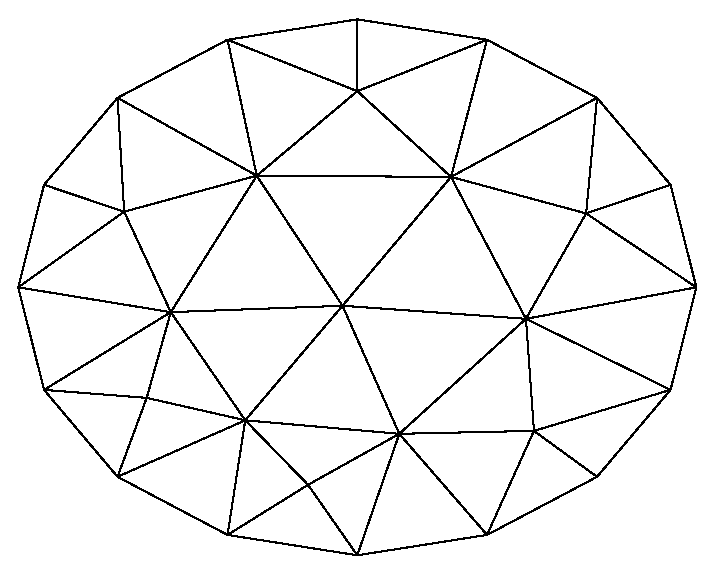
\includegraphics[width=0.35\textwidth]{cir0}}
      \vspace{0.2in}
      \subfloat{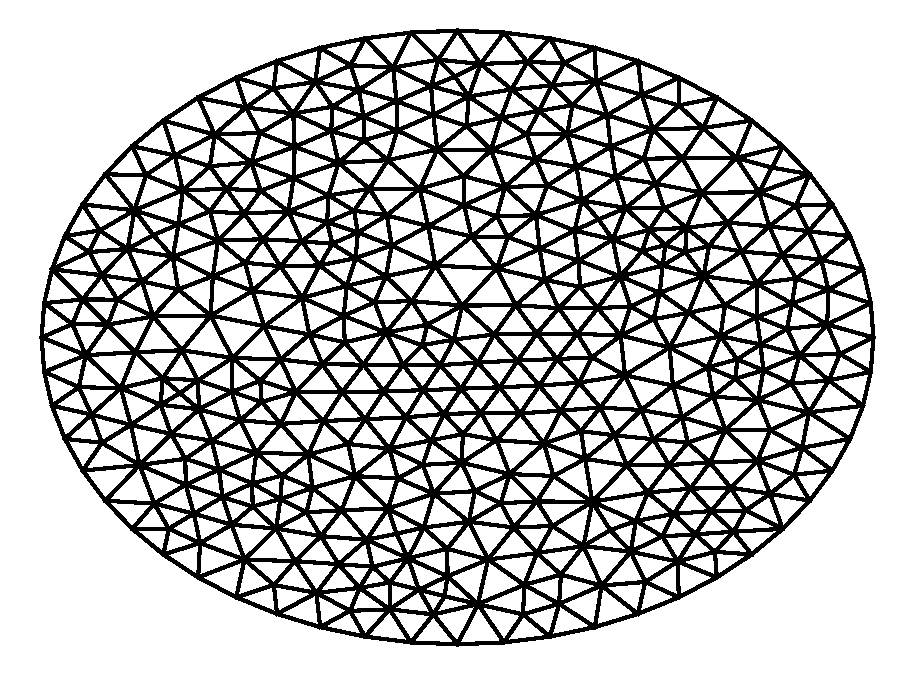
\includegraphics[width=0.35\textwidth]{cir2}}
      \caption{Mesh Refinement of Curved Mesh.}
      \label{fig:ch03_circle_meshes}
    \end{figure}
    
    \tref{tab:finite_cyl} shows that for refinement two, the refinement ratio is
    especially poor. However, for refinement three, the refinement ratio is
    roughly twice the expected rate.  Therefore, on average, the flux appears to
    be converging at the correct rate despite difficulties with mesh
    regeneration.

    \begin{table}
      \caption{Finite Cylinder Convergence Study Results.}
      \label{tab:finite_cyl}
      \begin{center}
        \begin{threeparttable}
        \begin{tabular}{cccccccccc}
          \toprule
          Refine & $\keff$ & $\keff$ error \units{\glsentryshort{pcm}} & $\keff$ ratio & \gls{rms} & 
            \gls{rms} ratio  & $\|e\|_{\infty}$ & $\|e\|_{\infty}$ ratio \\
          \midrule
          0     &0.895108&10160.26&4.18   &5.34E-02&2.57     &2.12E-01&1.62\\
          1     &0.972412&2429.90 &4.16   &2.07E-02&3.19     &1.31E-01&4.65\\
          2\tnote{$\dagger$}     &0.990870&584.06  &3.90   &6.50E-03&1.85     &2.81E-02&1.79\\
          3     &0.995215&149.61  &3.99   &3.51E-03&9.22     &1.57E-02&8.28\\
          4     &0.996336&37.48   &       &3.81E-04&         &1.90E-03&    \\
          Ref. & 0.996711 \\
          \bottomrule
        \end{tabular}
          \begin{tablenotes}
          \item[$\dagger$] Refinement ratio $\approx 1$ but next case $\approx
            8$.\\
            This is due to the movement of mesh nodes in the process of circular
            mesh regeneration.
          \end{tablenotes}
        \end{threeparttable}
      \end{center}
    \end{table}

\section{Two-Dimensional Benchmark Solutions}
  \label{sec:two_dimensional_benchmark_solutions}
  The work presented in this section was designed simulate nuclear power
  reactors with special attention to fast reactor applications.  Though the
  target application is fast reactors, the general solution of the diffusion
  equation is applicable to any reactor type to which the diffusion
  approximation applies. For example, VVER reactors are thermal reactors but
  have a hexagonal geometry.
  
  In this section, two-dimension nuclear reactor benchmark
  problems have been examined.  These problems come from existing benchmarks
  based on hexagonal geometry. Initial refinement is based on six triangles per
  hexagon and these triangles are split with each refinement. This collection of
  benchmarks represents various energy group structures, geometries, assembly
  sizes, boundary conditions, as well as other properties. Data used in these
  problems is concisely presented in \apref{ap:benchmarks}. Mesh refinement
  studies are provided and convergence is observed relative to the reference
  \keff value similar to analytic problems. 
  
  \subsection{VVER440}
    Proposed by \textcite{chao} and described in
    \sref{sec:vver440}, this benchmark is a two-dimensional hexagonal problem
    based on a VVER-440 reactor. The VVER-440 is a \gls{lwr} and, as such, 
    operates principally with thermal neutron spectrum. Cross sections are
    provided for a two-group energy structure.
    
    Power comparison between the most refined mesh and the reference solution
    are presented graphically in \fref{fig:diffusion_vver440}. Numerical mesh
    convergence study for the quantity $\keff$ is presented in
    \tref{tab:vver440}.

    \begin{figure}
      \centering
      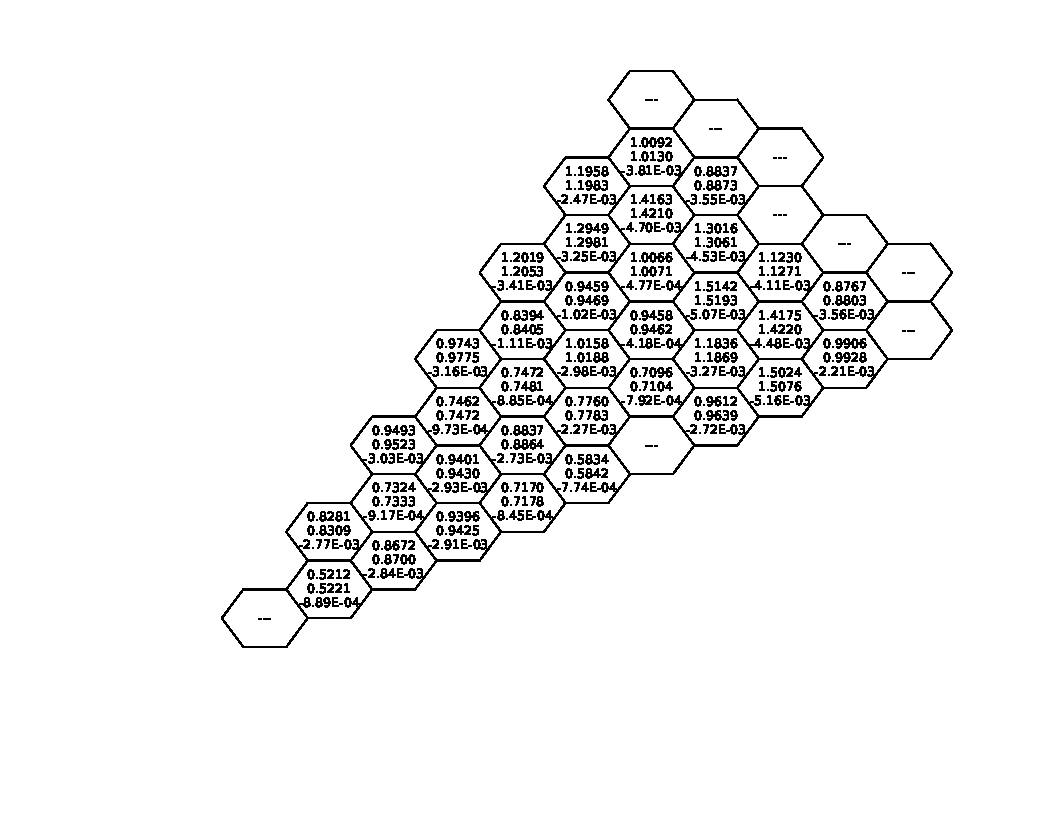
\includegraphics[width=\textwidth]{diffusion_vver440}
      \caption{VVER440 Benchmark Power Comparison for Most Refined Mesh.}
      \label{fig:diffusion_vver440}
      \Put(-125,500){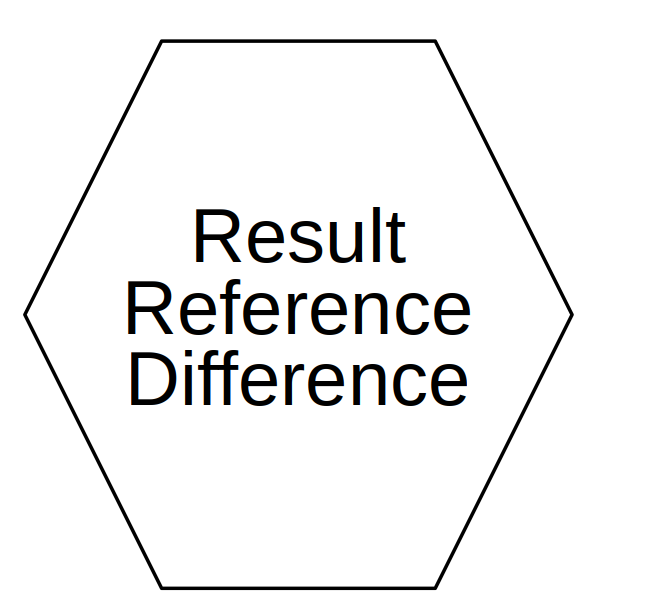
\includegraphics[width=0.10\textwidth]{hex_description}}
    \end{figure}

    \begin{table}
      \begin{center}
        \caption{VVER440 Benchmark Convergence Study.}
        \label{tab:vver440}
        \begin{threeparttable}
          \begin{tabular}{cccc}
            \toprule
            Refine & $\keff$ & $\keff$ error \units{\glsentryshort{pcm}}\\
            \midrule
            \csvreader[
              late after line=\\,
              late after last line=\\,]
              {ch03_diffusionResults/data/vver440.csv}{}
              {\csvcoli & \csvcolvi & \csvcolvii}
            Ref.\tnote{$\dagger$}  & 1.009700 \\
            \bottomrule
          \end{tabular}
          \begin{tablenotes}
            \item[$\dagger$] See \cite{chao}.
          \end{tablenotes}
        \end{threeparttable}
      \end{center}
    \end{table}

  \subsection{SNR}
    Proposed in the Argonne Code Center Benchmark Problem Book
    \cite{argonneBenchmark} and described in \sref{sec:snr}, this benchmark is a
    two-dimensional problem based on the SNR reactor. The SNR is a \gls{sfr} and
    operates principally with fast neutrons. Cross sections are provided for a
    four-group energy structure.

    Power comparison between the most refined mesh and numerical solution given
    by \dif are presented graphically in \fref{fig:diffusion_snr} (the benchmark
    does not specify a power distribution). A numerical mesh convergence study 
    for the quantity $\keff$ is presented in \tref{tab:snr}.

    \begin{figure}
      \centering
      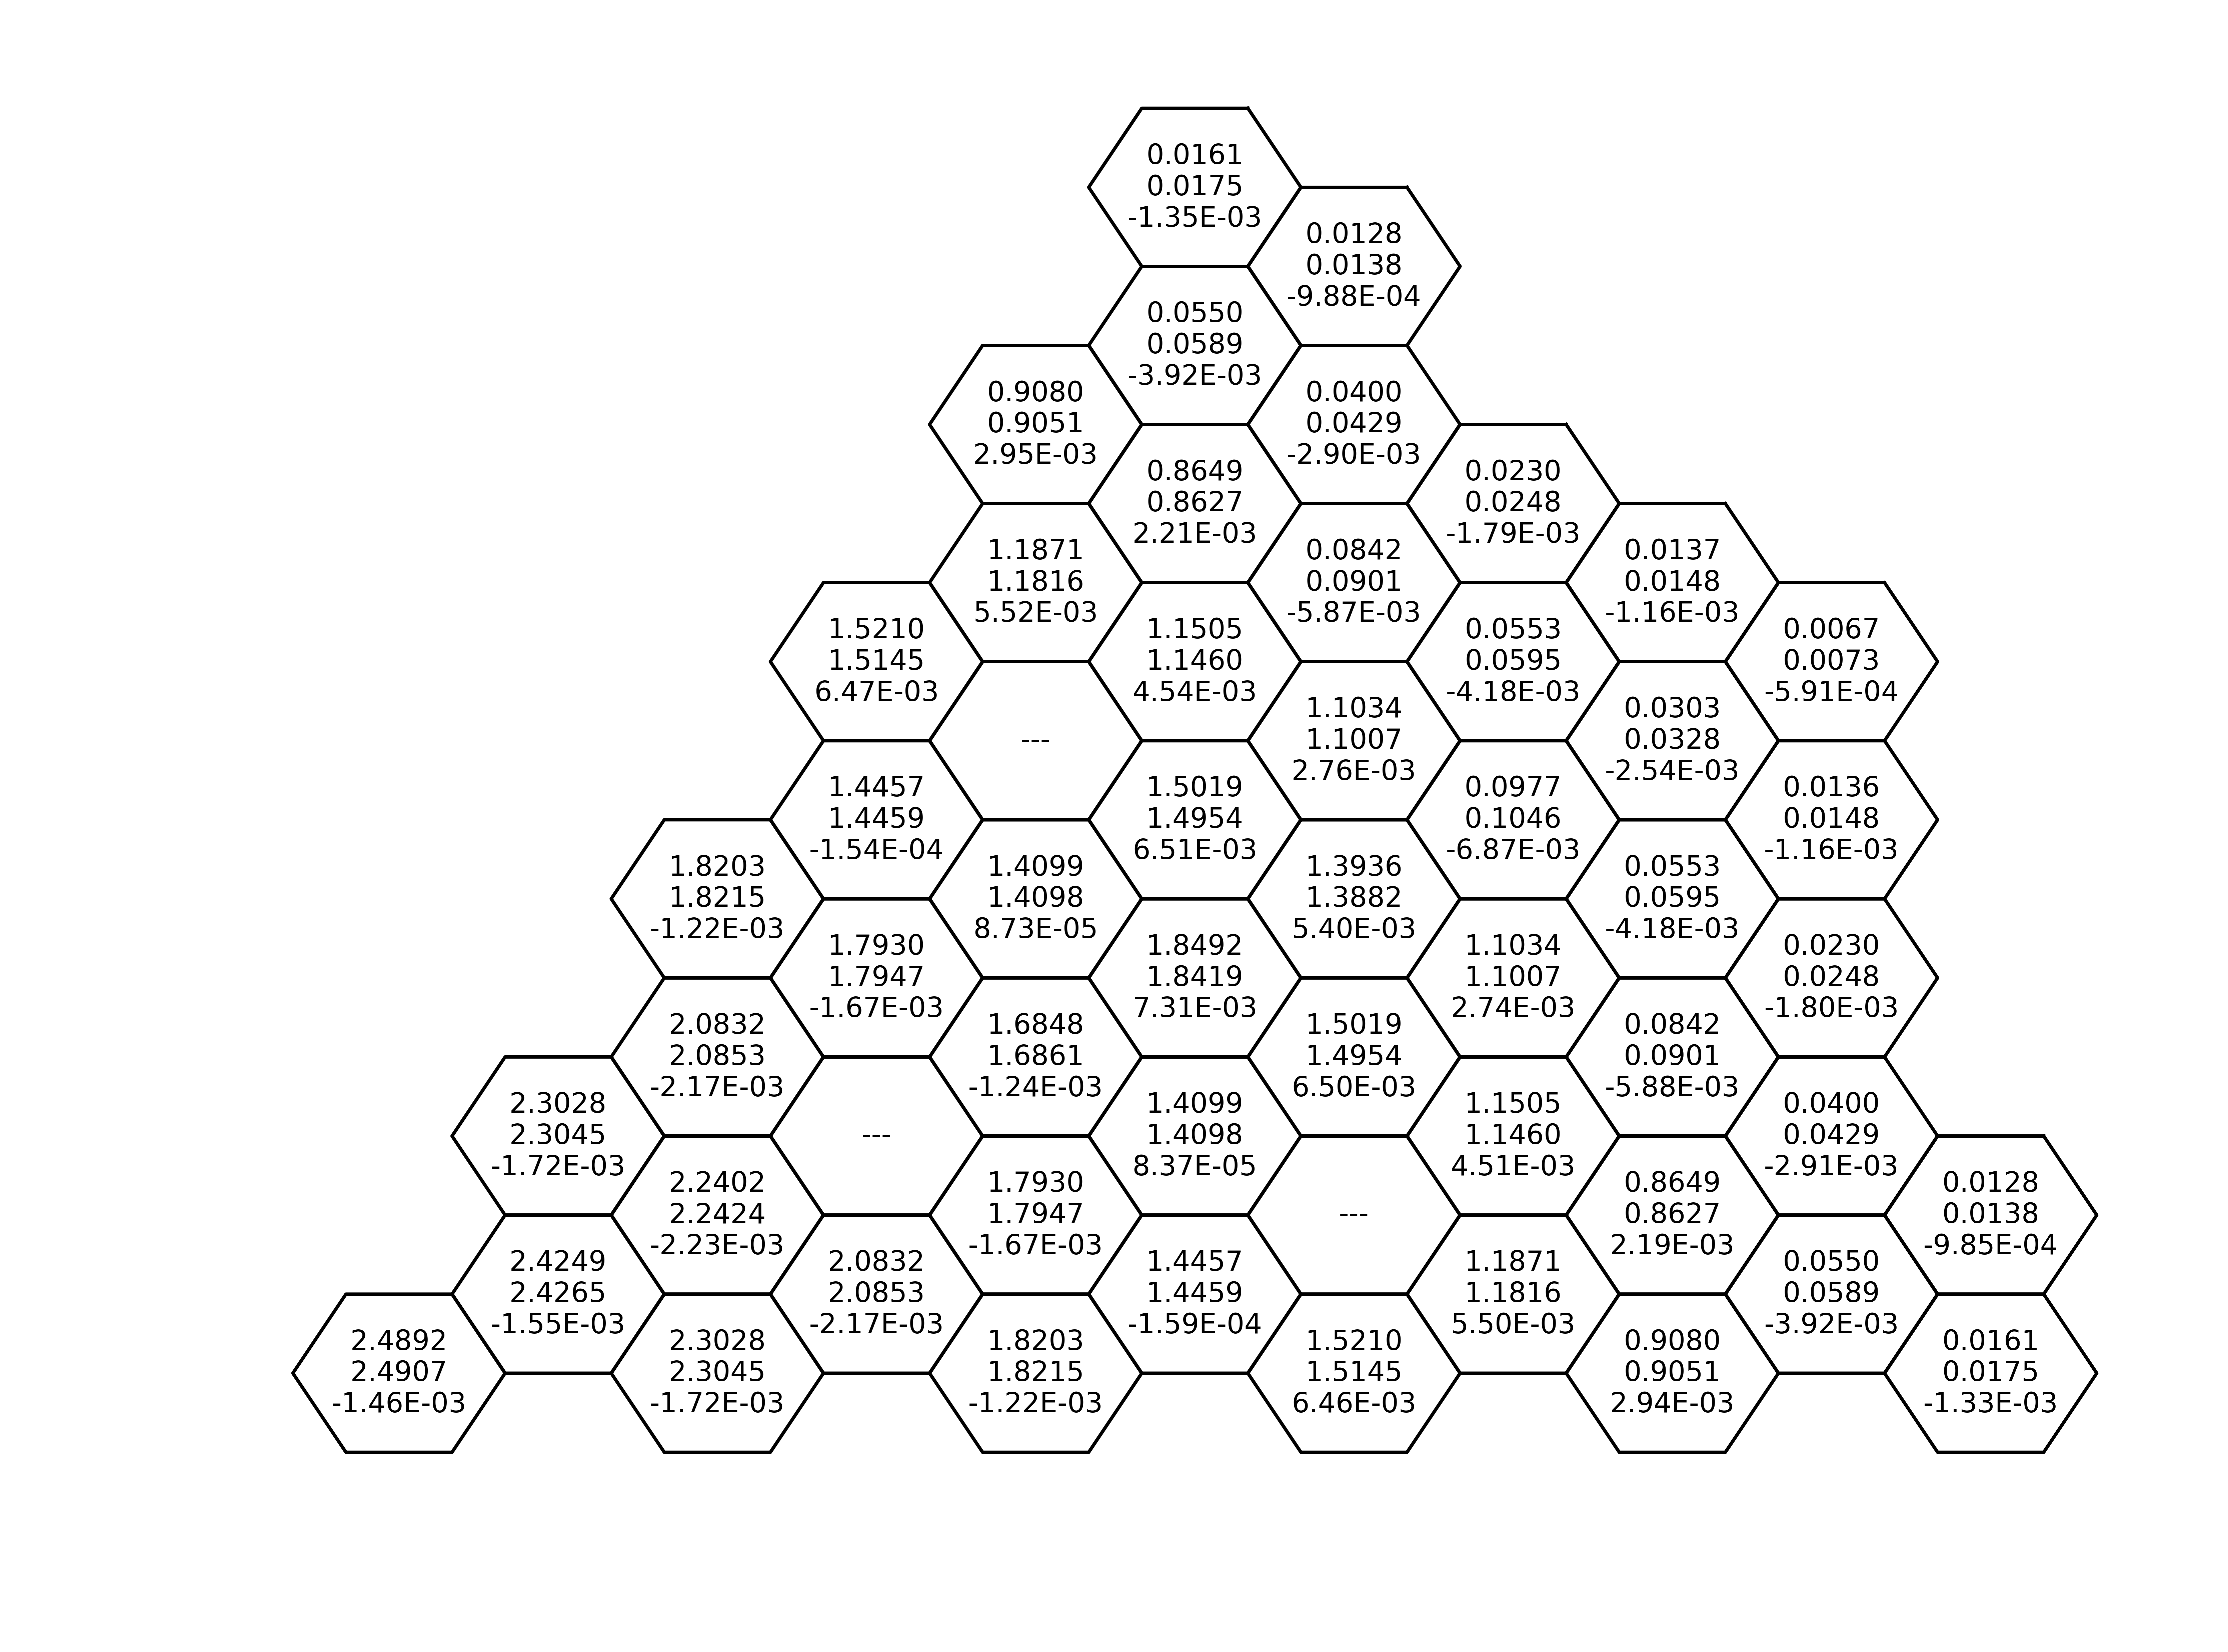
\includegraphics[width=\textwidth]{diffusion_snr}
      \caption{SNR Benchmark Power Comparison for Most Refined Mesh.}
      \label{fig:diffusion_snr}
      \Put(-125,550){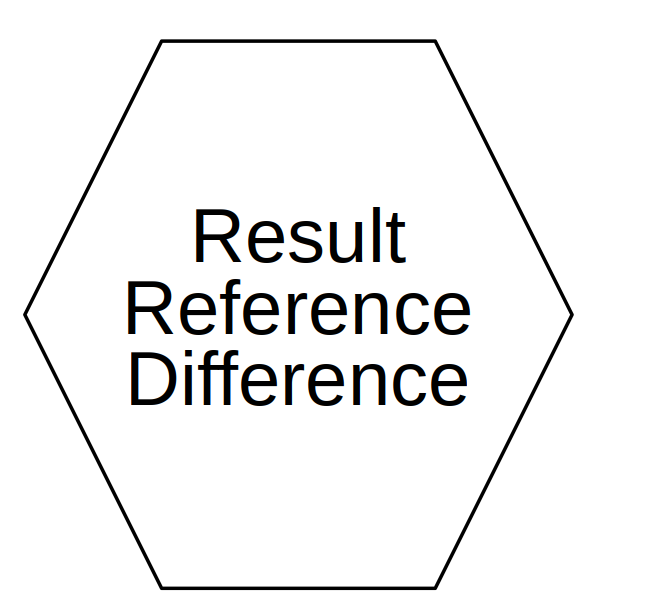
\includegraphics[width=0.10\textwidth]{hex_description}}
    \end{figure}
    
    \begin{table}
      \begin{center}
        \caption{SNR Benchmark Convergence Study.}
        \label{tab:snr}
        \begin{threeparttable}
          \begin{tabular}{cccc}
            \toprule
            Refine & $\keff$ & $\keff$ error \units{\glsentryshort{pcm}}\\
            \midrule
            \csvreader[
              late after line=\\,
              late after last line=\\,]
              {ch03_diffusionResults/data/snr.csv}{}
              {\csvcoli & \csvcolvi & \csvcolvii}
            Ref. \tnote{$\dagger$} & 1.124 \\
            \bottomrule
          \end{tabular}
          \begin{tablenotes}
            \item[$\dagger$] See \cite{argonneBenchmark}.
          \end{tablenotes}
        \end{threeparttable}
      \end{center}
    \end{table}

  \subsection{\texorpdfstring{\glsentryshort{hwr}}{HWR}}
    Proposed by \textcite{chao} and described in \sref{sec:hwr}, 
    this benchmark is a two-dimensional problem based on a large \gls{hwr}. This 
    is a heavy water moderated reactor and operates principally with thermal 
    neutrons. Cross sections are provided for a two-group energy structure.

    Power comparison between the most refined mesh and the reference solution
    are presented graphically in \fref{fig:diffusion_hwr}. A
    numerical mesh convergence study for the quantity $\keff$ is presented in
    \tref{tab:hwr}.

    \begin{figure}
      \centering
      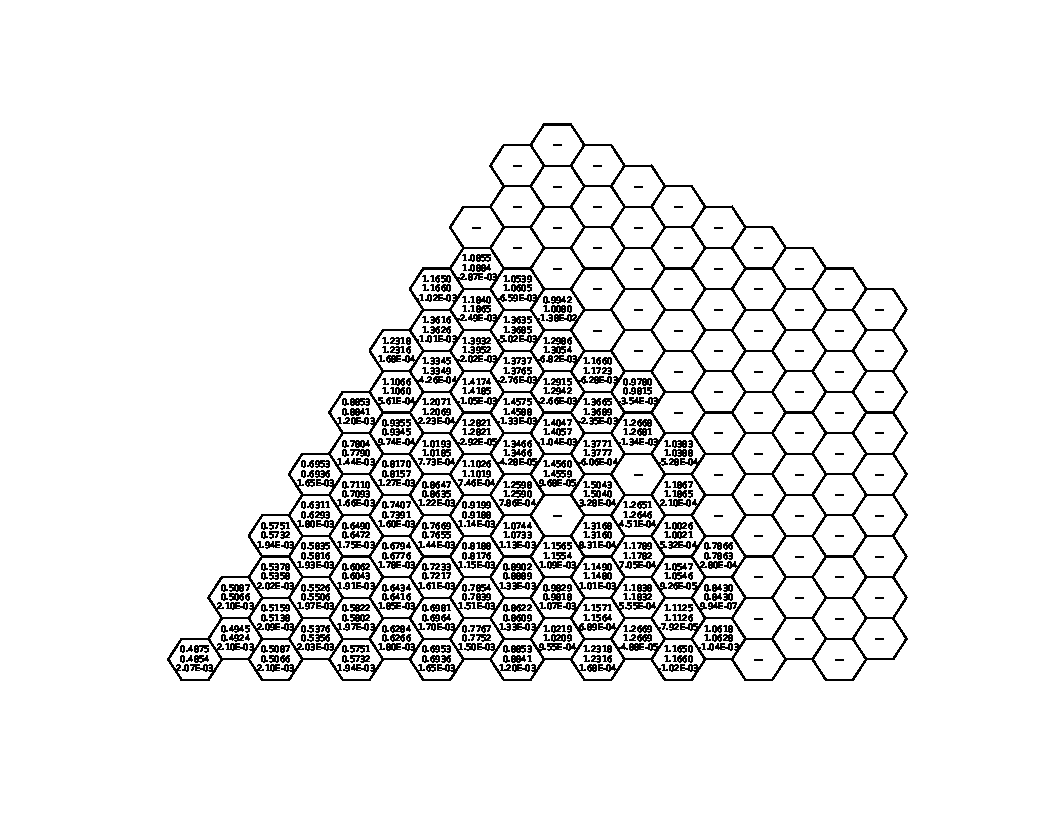
\includegraphics[width=\textwidth]{diffusion_hwr}
      \caption{\glsentryshort{hwr} Benchmark Power Comparison for Most Refined 
        Mesh.}
      \label{fig:diffusion_hwr}
      \Put(-125,500){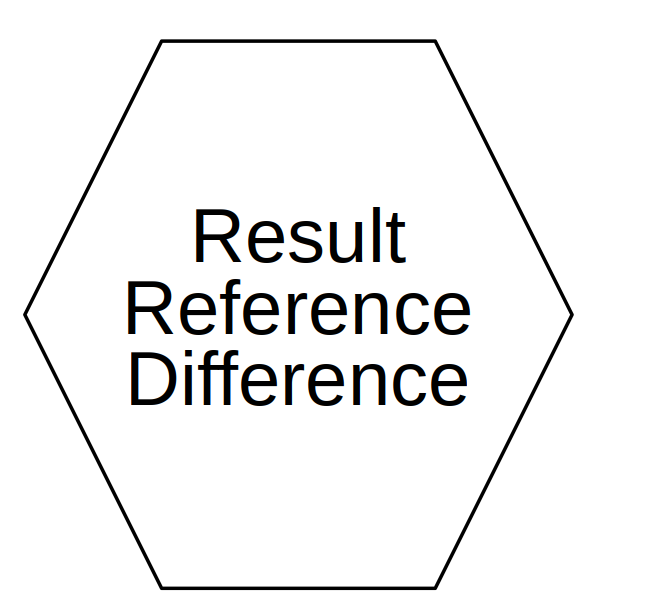
\includegraphics[width=0.10\textwidth]{hex_description}}
    \end{figure}

    \begin{table}
      \begin{center}
        \caption{\glsentryshort{hwr} Benchmark Convergence Study.}
        \label{tab:hwr}
        \begin{threeparttable}
          \begin{tabular}{cccc}
            \toprule
            Refine & $\keff$ & $\keff$ error \units{\glsentryshort{pcm}}\\
            \midrule
            \csvreader[
              late after line=\\,
              late after last line=\\,]
              {ch03_diffusionResults/data/hwr.csv}{}
              {\csvcoli & \csvcolvi & \csvcolvii}
            Ref.\tnote{$\dagger$} & 0.991965  \\
            \bottomrule
          \end{tabular}
          \begin{tablenotes}
            \item[$\dagger$] See \cite{chao}.
          \end{tablenotes}
        \end{threeparttable}
      \end{center}
    \end{table}

  \subsection{IAEA Hex}
    Proposed by \textcite{chao} and described in \sref{sec:iaea}, this
    two-dimensional problem was originally based on a two-dimensional \gls{pwr}
    with a Cartesian grid. The benchmark was converted to hexagonal geometry to
    represent a VVER reactor \cite{chao}. As it is originally based on a
    \gls{pwr} design, the reactor operates principally with a thermal neutron
    spectrum. Cross sections are provided for a two-group energy structure.

    The IAEA Hex reactor is presented in four scenarios; both with and without
    reflective assemblies as well as with albedo boundary condition 
    $\albedo = 0.125$ and $\albedo = 0.5$. Numerical mesh convergence studies
    are presented for the quantity $\keff$ for each case in each of
    \tref{tab:iaea_nore0125}, \tref{tab:iaea_nore0500},
    \tref{tab:iaea_refl0125}, and \tref{tab:iaea_refl0500}.

    % nore0125
    \begin{table}
      \begin{center}
        \caption{IAEA Hex Benchmark Convergence Study. No Reflector. $\albedo = 
          0.125$.}
        \label{tab:iaea_nore0125}
        \begin{threeparttable}
          \begin{tabular}{cccc}
            \toprule
            Refine & $\keff$ & $\keff$ error \units{\glsentryshort{pcm}} & $\keff$ ratio \\
            \midrule
            \csvreader[
              late after line=\\,
              late after last line=\\,]
              {ch03_diffusionResults/data/iaea_nore0125.csv}{}
              {\csvcoli & \csvcolvi & \csvcolvii}
            Ref. \tnote{$\dagger$} & 0.991378 \\
            \bottomrule
          \end{tabular}
          \begin{tablenotes}
            \item[$\dagger$] See \cite{chao}.
          \end{tablenotes}
        \end{threeparttable}
      \end{center}
    \end{table}

    % nore0500
    \begin{table}
      \begin{center}
        \caption{IAEA Hex Benchmark Convergence Study. No Reflector. $\albedo = 
          0.500$.}
        \label{tab:iaea_nore0500}
        \begin{threeparttable}
          \begin{tabular}{cccc}
            \toprule
            Refine & $\keff$ & $\keff$ error \units{\glsentryshort{pcm}}\\
            \midrule
            \csvreader[
              late after line=\\,
              late after last line=\\,]
              {ch03_diffusionResults/data/iaea_nore0500.csv}{}
              {\csvcoli & \csvcolvi & \csvcolvii}
            Ref. \tnote{$\dagger$} & 0.978077 \\
            \bottomrule
          \end{tabular}
          \begin{tablenotes}
            \item[$\dagger$] See \cite{chao}.
          \end{tablenotes}
        \end{threeparttable}
      \end{center}
    \end{table}

    % refl0125
    \begin{table}
      \begin{center}
        \caption{IAEA Hex Benchmark Convergence Study. With Reflector. $\albedo = 
          0.125$.}
        \label{tab:iaea_refl0125}
        \begin{threeparttable}
          \begin{tabular}{cccc}
            \toprule
            Refine & $\keff$ & $\keff$ error \units{\glsentryshort{pcm}}\\
            \midrule
            \csvreader[
              late after line=\\,
              late after last line=\\,]
              {ch03_diffusionResults/data/iaea_refl0125.csv}{}
              {\csvcoli & \csvcolvi & \csvcolvii}
            Ref. \tnote{$\dagger$} & 1.006630 \\
            \bottomrule
          \end{tabular}
          \begin{tablenotes}
            \item[$\dagger$] See \cite{chao}.
          \end{tablenotes}
        \end{threeparttable}
      \end{center}
    \end{table}

    % refl0500
    \begin{table}
      \begin{center}
      \caption{IAEA Hex Benchmark Convergence Study. With Reflector. $\albedo = 
        0.500$.}
      \label{tab:iaea_refl0500}
        \begin{threeparttable}
          \begin{tabular}{cccc}
            \toprule
            Refine & $\keff$ & $\keff$ error \units{\glsentryshort{pcm}} & $\keff$ ratio \\
            \midrule
            \csvreader[
              late after line=\\,
              late after last line=\\,]
              {ch03_diffusionResults/data/iaea_refl0500.csv}{}
              {\csvcoli & \csvcolvi & \csvcolvii}
            Ref. \tnote{$\dagger$} & 1.005507 \\
            \bottomrule
          \end{tabular}
          \begin{tablenotes}
            \item[$\dagger$] See \cite{chao}.
          \end{tablenotes}
        \end{threeparttable}
      \end{center}
    \end{table}

\section{Three-Dimensional Benchmark Solutions}
  \label{sec:three_dimensional_benchmark_solutions}
  For two-dimensional benchmarks, mesh refinement studies are provided and
  convergence is observed relative to the reference $\keff$ value similar to
  analytic problems. For three-dimensional benchmarks, control rod worth
  measurement is used to observe agreement of the \gls{fem} neutron diffusion
  solution to the benchmark solution. To measure control rod worth, three cases
  are run $\{A,B,C\}$ with control rods fully removed in case $A$, partially
  inserted in case $B$, and fully inserted in case $C$. Rod worth is presented
  in units \units{$\Delta k$} and calculated as 
  \begin{equation}
    \label{eq:rodworth}
    \text{Rod Worth}_x \units{$\Delta k$} = \frac{\keffsub{A} - \keffsub{x}}
      {\keffsub{A} \, \keffsub{x}}
  \end{equation}
  for $x = \{B,C\}$. That is, rod worth is always compared to the case with
  control rods fully removed, case $A$. Additionally, Rod Difference is
  presented in units \units{$\% \Delta$k} as
  \begin{equation}
    \label{eq:roddifference}
    \text{Rod Difference}_x \units{$\% \Delta k$} = (\keffsub{A} - \keffsub{x}) 
      \times 100 \%
  \end{equation}
  for $x = \{B,C\}$.

  \subsection{MONJU}
    Proposed by \textcite{monjuBenchmark} and described in 
    \sref{sec:monju}, this three-dimension fast reactor benchmark problem is 
    based on an \gls{sfr} operating principally with fast neutrons. Cross 
    sections are provided for a three-group energy structure. However, the 
    fission spectrum, $\chi$, is not provided in the specifications. 
    Instead, a fission spectrum is selected for benchmark agreement. This 
    assumed fission spectrum is presented in \tref{tab:monjuchi}. The rod worth 
    measurements appear insensitive to the choice of fission spectrum. 

    Reference data can be found in \tref{tab:monjukref}. Results from the
    \gls{fem} implementation are presented in \tref{tab:monju}. The error
    (difference between reference and calculated results) are presented in
    parenthesis next to the quantities. Rod worth is presented as calculated in
    \eref{eq:rodworth}. Rod difference is presented as calculated in
    \eref{eq:roddifference}.

    \begin{table}
      \begin{center}
        \caption{MONJU Benchmark Rod Worth Results.}
        \label{tab:monju}
        \begin{threeparttable}
          \begin{tabular}{ccll}
            \toprule
            Pattern & $\keff$ & Rod Worth \units{$\Delta k$} & 
              Rod Difference \units{\%$\Delta k$} \\
            \midrule
            A&1.056816&               &            \\
            B&1.031623&0.023 (2.51E-5) \tnote{$\dagger$} &2.52 (-0.07)\\
            C&1.006519&0.047 (1.77E-3)&5.03 (0.04) \\
            \bottomrule
          \end{tabular}
          \begin{tablenotes}
            \item[$\dagger$] Value in parentheses is difference to reference
              value from \cite{monjuBenchmark} as presented in 
              \sref{sec:monju}.
          \end{tablenotes}
        \end{threeparttable}
      \end{center}
    \end{table}
  
  \subsection{KNK}
    Proposed by \textcite{takedaBenchmark} and described in \sref{sec:knk}, this
    three-dimension benchmark problem is based on an \gls{sfr} and is a model of
    the KNK-II core. Cross sections are provided in a four-group energy
    structure. There are many materials specified in the problem so it also aids
    in testing material mapping in the code.  The reference data is for a
    solution to the neutron \textit{transport} equation. In this work, the cross
    sections from the transport problem are used to solve the neutron diffusion
    equation. This explains some of the numerical differences in the results but
    general trends are reflected. 

    Reference data can be found in \tref{tab:knkkref}. Results from the
    \gls{fem} neutron diffusion solution are presented in \tref{tab:knk}. The
    error (difference between reference and calculated results) are presented in
    parenthesis next to the quantities. Rod worth is presented as calculated in
    \eref{eq:rodworth}. Rod difference is presented as calculated in
    \eref{eq:roddifference}.

    \begin{table}
      \begin{center}
        \caption{KNK Benchmark Rod Worth Results.}
        \label{tab:knk}
        \begin{threeparttable}
          \begin{tabular}{ccll}
            \toprule
            Pattern & $\keff$ & Rod Worth \units{$\Delta k$} & 
              Rod Difference \units{\%$\Delta k$} \\
            \midrule
            A&1.061752&               &            \\
            B&0.942404&0.119 (1.55E-2) \tnote{$\dagger$} &11.93 (0.75)\\
            C&0.829829&0.263 (3.99E-2)&23.19 (1.67)\\
            \bottomrule
          \end{tabular}
          \begin{tablenotes}
            \item[$\dagger$] Value in parentheses is difference to reference
              value from \cite{takedaBenchmark} as presented in 
              \sref{sec:knk}.
          \end{tablenotes}
        \end{threeparttable}
      \end{center}
    \end{table}
